\documentclass[11pt]{article}
\usepackage{acl2015}
\usepackage{times}
\usepackage{url}
\usepackage{latexsym}
\usepackage{graphicx}
\usepackage{color}
%\setlength\titlebox{5cm}

% You can expand the titlebox if you need extra space
% to show all the authors. Please do not make the titlebox
% smaller than 5cm (the original size); we will check this
% in the camera-ready version and ask you to change it back.


\title{Zoom: a corpus of natural language descriptions of map locations}

\author{
	First Author \\
  Affiliation / Address 1 \\
  Affiliation / Address 2 \\
  Affiliation / Address 3 \\
  {\tt email@domain} \\
	\And
  Second Author \\
  Affiliation / Address 1 \\
  Affiliation / Address 2 \\
  Affiliation / Address 3 \\
  {\tt email@domain} \\
	\And
  Third Author \\
  Affiliation / Address 1 \\
  Affiliation / Address 2 \\
  Affiliation / Address 3 \\
  {\tt email@domain} \\
	\And
  Fourth Author \\
  Affiliation / Address 1 \\
  Affiliation / Address 2 \\
  Affiliation / Address 3 \\
  {\tt email@domain} \\
}
\date{}

\newenvironment{packed_enum}{
\begin{enumerate}
  \setlength{\itemsep}{1pt}
  \setlength{\parskip}{0pt}
  \setlength{\parsep}{0pt}
}{\end{enumerate}}



\begin{document}

\raggedbottom

\maketitle

\begin{abstract}
This paper describes 
an experiment  to elicit referring expressions
from human subjects 
for research in natural language generation and related fields,
and preliminary results of a computational model 
for the generation of these expressions.
\end{abstract}


%%%%%%%%%%%%%%%%%%%%%%%%%%%%%%%%%%%%%%%%	      
\section{Introduction}
%%%%%%%%%%%%%%%%%%%%%%%%%%%%%%%%%%%%%%%%	      

Referring Expression Generation (REG) is the computational task of producing adequate natural language descriptions (e.g., pronouns, definite descriptions, proper names, etc.) of domain entities. In particular, the issue of how to determine the semantic contents of definite descriptions (e.g., `the Indian restaurant on 5th street', `the restaurant we went to last night',  etc.) has received significant attention in the field, and it is also the focus of the present work.

Existing approaches to REG largely consist of algorithmic solutions, many of which have been influenced by, or adapted from, the Dale \& Reiter Incremental algorithm in \cite{incremental}. The use of machine learning (ML) techniques, by contrast, seems to be less frequent than in other NLG tasks and in related fields, although a number of exceptions do exist (e.g., \cite{jordan,speaker-dependent,viethen-phd,garoufi13,thiago-svm}). 

A possible explanation for the small interest in ML for REG may be the relatively low availability of data. While research in many fields may benefit from the wide availability of text corpora (e.g., obtainable from the web), research in REG usually requires highly specialised data  - hereby called REG corpora - conveying not only referring expressions produced by human speakers, but also a fully-annotated representation of the context (i.e., all objects and their semantic properties) within which the expressions have been produced. 

Examples of REG corpora include TUNA \cite{tuna-corpus}, GRE3D3 \cite{gre3d3}, and Stars \cite{stars-mutual-disamb}. Despite the usefulness of these resources for a large body of work, however, the available descriptions are still at some distance from those normally observed in more realistic applications, and in any case further research questions will usually require new data. 

In this paper we present the Zoom corpus of referring expressions. Zoom addresses a domain that is considerably closer to real-world applications \textcolor{blue}{than existing work}(namely, city maps in different degrees of detail represented by zoom levels), involving both singular and plural reference, and making extensive use of relational properties. Moreover, Zoom descriptions were produced by both Spanish and Portuguese speakers, which will allow (to the best of our knowledge, for the first time) a comprehensive study of the REG surface realisation subtask in these languages, and enable research on the issues of human variation in REG \cite{trainable-speaker,romina-coling,non-det}. 


%%%%%%%%%%%%%%%%%%%%%%%%%%%%%%%%%%%%%%%%	       
\section{Related work}
%%%%%%%%%%%%%%%%%%%%%%%%%%%%%%%%%%%%%%%%	       
\label{sec-background}

TUNA \cite{tuna-corpus} was the first prominent REG corpus to be made publicly available for research purposes. The corpus was developed in a series of controlled experiments, containing 2280 atomic descriptions produced by 60 speakers in two domains (1200 descriptions of furniture items and 1080 descriptions of people's photographs). 

GRE3D3 and its extension GRE3D7 \cite{gre3d3,gre3d7} were developed in a series of web-based experiments primarily focussed on the study of relational descriptions. GRE3D3 contains 630 descriptions produced by 63 speakers, and GRE3D7 contains 4480 descriptions produced by 287 speakers. The domain consists of simple visual scenes containing only two kinds of objects (boxes and spheres).

Stars \cite{stars-mutual-disamb} and its extension Stars2 were collected for the study of referential overspecification. Stars contains 704 descriptions produced by 64 speakers in a web-based experiment. Stars2 was produced in dialogue situations involving subject pairs, and it contains 884 descriptions produced by 56 speakers. Both domains make use of simple visual scenes containing up to four object types (e.g., stars, boxes, cones and spheres) and include atomic and relational descriptions alike. 



%%%%%%%%%%%%%%%%%%%%%%%%%%%%%%%%%%%%%%%%	       
\section{Experiment}
%%%%%%%%%%%%%%%%%%%%%%%%%%%%%%%%%%%%%%%%	       
\label{sec-experiment}

We designed a web-based experiment to collect natural language descriptions of map locations in both Spanish and Portuguese. The collected data set comprises a corpus of referring expressions for research in REG and related fields. The situations of reference under consideration make use of map scenes in two degrees of detail (represented by low and high zoom levels), and address instances of singular and plural reference. A fragment of the experiment interface is shown in Fig. \ref{fig-interface}.

\begin{figure}[ht]
\begin{center}
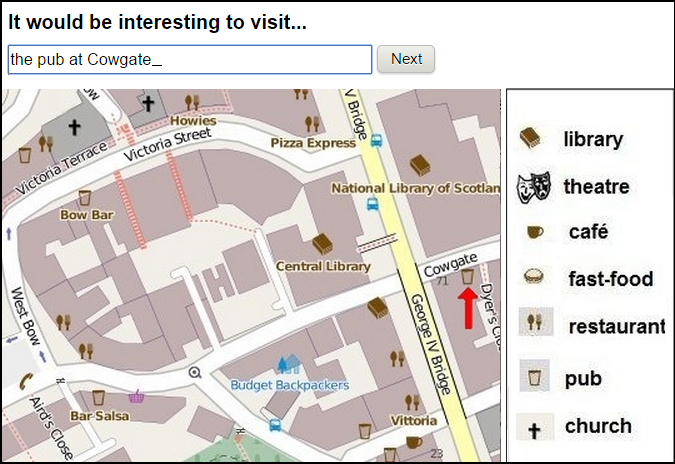
\includegraphics[width=7.6cm]{figures/interface.png}\\[0pt]
\caption{Experiment interface}
\label{fig-interface}
\end{center}
\end{figure}

{\bf Subjects:} Volunteers were recruited upon  invitation sent by email. The Portuguese portion of the corpus had 93 participants, being 66 (71.0\%) male and 27 (29.0\%) female. The Spanish corpus had 80 participants, being 59 male (69.4\%) and 26 female (30.6\%).

{\bf Procedure:} Subjects received a web link to the on-line experiment interface (cf. Fig. \ref{fig-interface}) with self-contained instructions. Age and gender details were collected for statistical purposes. The experiment consisted of a series of map images presented in random order, one by one. Each map scene showed a particular location (e.g., a restaurant, pub, theatre etc.) pointed by an arrow. For each scene, subjects were required to imagine that they were giving travel advice to a friend, and to complete the sentence `It would be interesting to visit...' with a description of the location pointed by the arrow. After pressing a `Next' button, another stimulus was selected at random until the end of the experiment. The first two images were fillers solely intended to make subjects familiar with the experiment setting, and the corresponding responses were not recorded. Incomplete trials, and ill-formed descriptions, were also discarded. 

{\bf Materials:} The experiment made use of the purpose-built interface illustrated in Fig. \ref{fig-interface}, and a set of map images obtained from OpenStreetMap\footnote{\url{openstreetmap.org}}, which consisted of selected portions of maps of Madrid and Lisbon,  \textcolor{blue}{we select those cities because the most of participants it suppose to live in Argentina or Brazil, and we want to select a city with the same language but unknown places for the participants, in order to not receive things as... ``The bar we went last night''} . For each city, 10 map locations were used. Each location was shown in low and high zoom levels, making 20 images in total. In both cases, the intended target was kept the same, but the more detailed version would display a larger number of distractors and additional details in general. In addition to that, certain street and landmark names might not be depicted at different zoom levels. Half images showed a single arrow pointing to one map location (i.e., requiring a single description as `the restaurant on Baker street'), whereas the other half showed two arrows pointed to two different locations (and hence requiring a reference to a set, as in `the two restaurants near the museum'\textcolor{blue}{ or `The restaurante near to museum and the restaurante in front to the Bank'}). 

{\bf Data collection:} Upon manual verification, 602 ill-formed Portuguese descriptions and 366 Spanish descriptions were discarded. Thus, the Portuguese subcorpus consists of 1358 descriptions, and the Spanish subcorpus consists of 1234 descriptions. In the Portuguese subcorpus, 78.6\% of the descriptions include relational properties. In addition to that, 36.4\% were minimally distinguishing, 44.3\% were overspecified, and  19.3\% were underspecified. In the Spanish subcorpus, 70\% of the descriptions include relational properties, 35\% were minimally distinguishing, 40\% were overspecified, and 25\% were underspecified. Underspecified descriptions are not common in existing REG corpora (certainly not in this proportion), which may reflect the complexity of the domain.

{\bf Annotation:} Each referring expression was modelled \textcolor{blue}{as maximum with} a set of 26 attributes \textcolor{blue}{wich are 10 for the target object and 4 for each of the landmaks objects considering 4 landmarks (maybe we should to justify here why)}. In the case of plural descriptions (i.e., those involving two target objects), this attribute set was doubled. Every object was annotated with the atomic attributes {\em type}, {\em name} and {\em others} and, in the case of landmark objects, also with their {\em id}. In addition to that, seven relational properties were considered: {\em in/on/at}, {\em next-to}, {\em right-of}, {\em left-of}, {\em in-front-of}, {\em behind-of}, and the multivalue relation {\em between}. The collected descriptions were fully annotated by two independent annotators. After completion, a third annotator assumed the role of judge and provided the final annotation. Since the annotation scheme was fairly straightforward (i.e., largely because all non-standard responses were simply assigned to the {\em others} attribute), agreement between judges as measured by Kappa \cite{kappa} was 84\% at the attribute level. Both referential contexts and referring expressions were represented in XML format using a relational version of the XML format adopted in the TUNA corpus \cite{tuna-corpus}. 

{\bf Comparison with previous work:} Table \textcolor{blue}{\ref{tab-comparison-f} and }\ref{tab-comparison} presents a comparison between the collected data and existing REG corpora. \textcolor{blue}{\ref{tab-comparison-f} shows the principal features comparison, those are, count of RE, count of participants, language selected, if has references to plurals, and if has zoom levels of details into account\footnote{En. for English, Pt. for Portuguese, Sp. for Spanish. TUNA-F. for TUNA-Furniture, and TUNA-P. for TUNA-people} and \ref{tab-comparison}}\footnote{The information on TUNA and Zoom descriptions is based on the singular portion of each corpus only}: the number of possible atomic attributes (Attrib.), the number of possible landmarks (LMs) in a  description, the average description size (in number of annotated properties), and the proportion of property usage, which is taken to be the proportion of properties that appear in the description over the total number of possible attributes and landmarks. From a REG perspective, larger description sizes and lower usage rates are likely to represent more complex situations of reference. \textcolor{blue}{Also all cited corpus are in English language, and our ZOOM corpus is of Spanish and Portuguese languages.}


\begin{table}[ht]
\begin{center}
\footnotesize{
\caption{Comparison features corpus with existing REG corpora}
\label{tab-comparison-f}
\begin{tabular} {  l c c c c c}
\hline
Corpus			& RE    & Partici-& Lan-  & Plural & Zoom \\
						&count  &pants    & guage &ref.    &      \\
\hline
TUNA-F.			& 1200	& 60	&	En.	& si  & no \\
TUNA-P.			& 1080	& 60	& En.	& si  & no \\
GRE3D3			&	630		& 63	& En.	& no  & no \\
GRE3D7			&	4480	& 287	& En.	& no  & no \\
Stars				&	704		& 64	& En.	& no  & no \\
Stars2			& 884		& 56	& En.	& no  & no \\
Zoom-Pt.		& 1358	& 93	& Pt.	& si  & si \\
Zoom-Sp.		& 1234	& 80	& Sp.	& si  & si \\
\hline
\end{tabular}
}
\end{center}
\end{table}



\begin{table}[ht]
\begin{center}
\footnotesize{
\caption{Comparison \textcolor{blue}{annotations} with existing REG corpora}
\label{tab-comparison}
\begin{tabular} {  l c c c c}
\hline
Corpus											& Attrib.			& LMs			& Avg.size	& Usage \\
\hline
TUNA-Furniture							& 4								& 0							&	3.1				& 0.8   \\
TUNA-People									& 10							& 0							& 3.1				& 0.3   \\
GRE3D3											&	9								& 1							& 3.4				& 0.3   \\
GRE3D7											&	6								& 1							& 3.0				& 0.4   \\
Stars												&	8								& 2							& 4.4				& 0.4   \\
Stars2											& 9								& 2							& 3.3				& 0.3   \\
Zoom-Portuguese							& 19							& 4							& 6.7				& 0.3   \\
Zoom-Spanish								& 19							& 4							& 7.2				& 0.3   \\
\hline
\end{tabular}
}
\end{center}
\end{table}


%%%%%%%%%%%%%%%%%%%%%%%%%%%%%%%%%%%%%%%%
\section{REG evaluation}
%%%%%%%%%%%%%%%%%%%%%%%%%%%%%%%%%%%%%%%%
\label{sec-eval}

In what follows we illustrate the use of the Zoom corpus as training and test data for a machine learning approach to REG adapted from \cite{thiago-svm}. The  goal of this evaluation is to provide reference results for future comparison with purpose-built REG algorithms, and not to present a complete REG solution for the Zoom domain or others.

The present model consists of 12 binary classifiers representing whether individual referential attributes should be selected for inclusion in an output description. The classifiers correspond to atomic attributes \textcolor{blue}{only} of the target and first landmark object ({\em type}, {\em name} and {\em others}), and relations. Referential attributes of other landmark objects were not modelled due to data sparsity and also to reduce computational costs. For similar reasons, the multivalue {\em between} relation is also presently disregarded, and `corner' relations involving two landmarks (e.g., two streets) will be modelled as two independent classification tasks.

Two learning features were considered by each classifier: {\em landmarkCount}, which represents the number of landmark objects near the main target, and {\em distractorCount}, which represents the number of objects of the same type as the target within the relevant context in the map.

From the outcome of the 12 binary classifiers, a description is built by considering atomic target attributes in the first place. All attributes that correspond to a positive prediction are selected for inclusion in the output description. Next, relations are considered. If no relation is predicted, the algorithm terminates by returning an atomic description  of the main target object. If the description includes a relation, the corresponding landmark object is selected, and the algorithm is called recursively to describe it as well. Since every attribute that corresponds to a positive prediction is always selected, the algorithm does not regard uniqueness as a stop condition. As a result, the output description may convey a certain amount of overspecification.

For evaluation purposes, we used the subset of singular descriptions from the Portuguese portion of the corpus, comprising 821 descriptions. Evaluation was carried out by comparing the corpus description with the system output to measure overall accuracy (i.e., the number of exact matches between the two descriptions), Dice \cite{dice} and MASI \cite{masi} coefficients.% (i.e., the degree of overlap between the algorithm output and the corresponding corpus description).

Following \cite{thiago-svm}, we built a REG model using support vector machines with radial basis function kernel. The classifiers were trained and tested using 6-fold cross validation. Optimal parameters were selected using grid search as follows: for each step in the main $k$-fold validation, one fold is reserved for testing, and the remaining $k-1$ folders are subject  to a secondary cross-validation procedure in which different parameter combinations are attempted. The $C$ parameter is assigned the values 1, 10, 100 and 1000, and $\gamma$ is assigned 1, 0.1, 0.001 and 0.0001. The best-performing parameter set is selected to build a classifier trained from the $k-1$ folders, and tested on the test data. This procedure is repeated for every iteration of the main cross-validation procedure.

Table \ref{tab-reg-results} summarises the results obtained by the REG algorithm built from SVM classifiers, those obtained by a baseline system representing a relational extension of the Dale \& Reiter Incremental Algorithm, and by a Random selection strategy.  

% these results are for SVM.All.VAR-   compared to the AEI- baseline
\begin{table}[ht]
\begin{center}
\caption{REG results}
\label{tab-reg-results}
\footnotesize{
\begin{tabular} {  l c c c }
\hline
{Algorithm}							& {Acc.} 	& { Dice}		& MASI \\ \hline 
SVM											& 0.15		&	0.51			& 0.28 \\
Incremental							& 0.04		&	0.53			& 0.21 \\
Random selection       	& 0.03    & 0.45      & 0.15 \\
\hline
\end{tabular}
}
\end{center}
\end{table}
\normalsize

We compare accuracy scores obtained by every algorithm pair using the chi-square test, and we compare {\em Dice} scores using {\em Wilcoxon's} signed-rank test. In terms of overall accuracy, the SVM approach outperforms both alternatives. The difference from the second best-performing algorithm (i.e., the Incremental approach) is significant ($\chi^{2}=$ 79.87, df=1, p$<$0.0001). Only in terms of Dice scores a small effect in the opposite direction is observed (T=137570.5, p$=$ 0.01413). 

We also assessed the performance of the individual classifiers. Table \ref{tab-svm-results} shows these results as measured by precision (P), recall (R), F1-measure (F1) and area under the ROC curve (AUC). 

%these are the rsults for the training over the set of ALL speakers 
\begin{table}[ht]
\begin{center}
\footnotesize{
\caption{Classifier results}
\begin{tabular}{l c c c c }
\hline
{{Classifier}}	& {P} & {R} & {$F_{1}$} & {AUC} \\
\hline
{{tg\_type}} 			& 0.95 & 1.00 & 0.98 & 0.25 \\
{{tg\_name}}			& 0.09 & 0.05 & 0.07 & 0.41 \\
{{tg\_other}}			& 0.00 & 0.00 & 0.00 & 0.05 \\                               
{{lm\_type}}			& 0.93 & 1.00 & 0.96 & 0.44 \\                               
{{lm\_name}}			& 0.97 & 1.00 & 0.98 & 0.35 \\                               
{{lm\_other}}			& 0.00 & 0.00 & 0.00 & 0.43 \\                               
{{next-to}}				& 0.50 & 0.24 & 0.32 & 0.63 \\                               
{{right-of}}			& 0.00 & 0.00 & 0.00 & 0.28 \\                               
{{left-of}}				& 0.00 & 0.00 & 0.00 & 0.27 \\                               
{{in-front-of}}		& 0.00 & 0.00 & 0.00 & 0.42 \\                               
{{behind-of}}			& 0.00 & 0.00 & 0.00 & 0.17 \\                               
{{in/on/at}} 			& 0.60 & 0.60 & 0.60 & 0.61 \\                               
\hline                   
\end{tabular}
\label{tab-svm-results}
}
\end{center}
\end{table}
\normalsize

From these results we notice that highly frequent attributes (e.g., type \textcolor{blue}{in the case of target object} and name \textcolor{blue}{for the landmark object}) were classified  with high accuracy, whereas others (e.g., multivalue attributes and relations) were not. 

%%%%%%%%%%%%%%%%%%%%%%%%%%%%%%%%%%%%%%%%	     
\section{Discussion}
%%%%%%%%%%%%%%%%%%%%%%%%%%%%%%%%%%%%%%%%	     
\label{sec-final}

This paper has introduced the Zoom corpus of natural language descriptions of map locations, a resource intended to support future research in REG and related fields. Preliminary results of a SVM-based approach to REG - which were solely presented for the future assessment of REG algorithms based on Zoom data - hint at the actual complexity of the REG task in this domain in a number of ways. First, we notice that a similar approach in \cite{thiago-svm} on GRE3D3 and GRE3D7 data has obtained considerably higher mean accuracy. This is partially explained by the increased complexity of the Zoom domain, but also by the currently  simple annotation scheme.

Second, we notice that Zoom descriptions are prone to convey relations between a single target and multiple landmark objects, as in `the restaurant between the 5th and 6th streets'. Although common in language use, the use of multiple relational properties in this way has been little investigated in the REG field. 

Finally, we notice that the Zoom domain contains two descriptions for every target object, which are based on different - but related - models corresponding to the same map location seen at different zoom levels. Interestingly, the referring expression in a 1X situation may or may not be the same as in a 2X situation. Changes of this kind are common in interactive applications (e.g., in which the context of reference may change in structure or in the number of objects and referable properties), and the challenge for REG algorithms would be to produced an appropriate description for the modified context without starting from scratch. REG algorithms based on local context partitioning \cite{areces08} may have an advantage in this respect, but further investigation is still required.


%..........................
\section*{Acknowledgements}
%..........................
This work has been supported by anonymous. 

\clearpage
\bibliographystyle{acl}
\bibliography{mainZoom}

\end{document}
